\documentclass[12pt,letterpaper]{article}
\usepackage[landscape,margin=1.25cm]{geometry}
\usepackage{fontspec}
\usepackage[provide=*,spanish]{babel}
\usepackage{xcolor}
\usepackage{graphicx}
\usepackage{booktabs}
\usepackage{tabularx}
\usepackage{hyperref}
\usepackage{array}
\usepackage{amsmath}
\IfFontExistsTF{DejaVu Sans}{\setmainfont{DejaVu Sans}}{\setmainfont{Arial}}
\definecolor{ElectricBlue}{HTML}{0066FF}
\definecolor{NeonCyan}{HTML}{00FFFF}
\definecolor{DarkGray}{HTML}{1E1E1E}
\definecolor{SoftBlue}{HTML}{EEF6FF}
\hypersetup{colorlinks=true,urlcolor=ElectricBlue}
\pagestyle{empty}
\setlength{\parindent}{0pt}
\newenvironment{slide}[1]{%
  \clearpage\noindent
  {\color{ElectricBlue}\fontsize{26}{30}\selectfont\bfseries #1\par}
  {\color{NeonCyan}\rule{\textwidth}{3pt}}\vspace{.45cm}
}{\vfill\hfill{\small\color{DarkGray}Laboratorio 6 · 22193 · \thepage}}
\newcommand{\card}[2]{\fcolorbox{ElectricBlue}{SoftBlue}{\begin{minipage}[c][2.15cm][c]{.28\textwidth}
\centering{\color{ElectricBlue}\fontsize{23}{26}\selectfont\bfseries #1}\par\small #2
\end{minipage}}}

\begin{document}

\pagecolor{DarkGray}\color{white}
\vspace*{1.1cm}
{\color{NeonCyan}\bfseries DEEP LEARNING 2026 · SECCIÓN 30\par}
\vspace{.65cm}
{\fontsize{38}{44}\selectfont\bfseries Calculadora Neuronal\par}
{\fontsize{24}{30}\selectfont Un repositorio reproducible de seq2seq y atención\par}
\vspace{.8cm}
\colorbox{ElectricBlue}{\parbox{.88\textwidth}{\color{white}\large
De la implementación de Bahdanau a un modelo de torneo con 97.20\% de exactitud.}}
\vfill
{\large Pablo Daniel Barillas Moreno · 22193}\par
\href{https://github.com/DanielBarillasM/Laboratorio-6_Daniel-Barillas_22193_DLYSI_Sec-30}{\color{NeonCyan}github.com/DanielBarillasM/Laboratorio-6\_Daniel-Barillas\_22193\_DLYSI\_Sec-30}
\clearpage\nopagecolor\color{DarkGray}

\begin{slide}{01 · Pregunta y entrega}
\begin{minipage}{.52\textwidth}
{\Large ¿Puede una red aprender a sumar y restar sin recibir reglas?}
\vspace{.4cm}
\begin{itemize}
\item Entrada textual: \texttt{4821+3976}.
\item Salida autoregresiva: \texttt{8797}.
\item Entrenamiento sintético con máximo cuatro cifras.
\item Comparación con/sin atención y una mejora controlada.
\item Cinco casos adversariales dentro del rango permitido.
\end{itemize}
\end{minipage}\hfill
\begin{minipage}{.42\textwidth}
\fcolorbox{ElectricBlue}{SoftBlue}{\parbox{.9\textwidth}{\centering\Large
Notebook ejecutado\\3 checkpoints\\7 figuras\\2 documentos PDF\\validación automatizada}}
\end{minipage}
\end{slide}

\begin{slide}{02 · Arquitectura}
\begin{center}
\fcolorbox{ElectricBlue}{SoftBlue}{\parbox{.2\textwidth}{\centering\bfseries Expresión\\carácter por carácter}}
$\longrightarrow$
\fcolorbox{ElectricBlue}{SoftBlue}{\parbox{.2\textwidth}{\centering\bfseries Embedding +\\GRU bidireccional}}
$\longrightarrow$
\fcolorbox{ElectricBlue}{SoftBlue}{\parbox{.2\textwidth}{\centering\bfseries Atención\\aditiva}}
$\longrightarrow$
\fcolorbox{ElectricBlue}{SoftBlue}{\parbox{.2\textwidth}{\centering\bfseries GRUCell +\\vocabulario}}
\end{center}
\vspace{.5cm}
\[
e_j=v^\top\tanh(W_qs+W_kh_j),\qquad
\alpha=\operatorname{softmax}(e),\qquad c=\sum_j\alpha_jh_j
\]
\begin{itemize}
\item La máscara asigna peso cero a \texttt{<PAD>}.
\item El contexto cambia en cada paso de salida.
\item 186,767 parámetros: 24.9\% del límite permitido.
\end{itemize}
\end{slide}

\begin{slide}{03 · Experimento controlado}
\begin{center}
\begin{tabular}{lccc}
\toprule & Atención & Sin atención & Torneo \\
\midrule
Ejemplos & 40,000 & 40,000 & 40,000 \\
Épocas & 15 & 15 & 15 \\
Dimensión oculta & 64 & 64 & 64 \\
Semilla & 2026 & 2026 & 2026 \\
Salida invertida & No & No & \textbf{Sí} \\
\bottomrule
\end{tabular}
\end{center}
\vspace{.45cm}
\fcolorbox{ElectricBlue}{SoftBlue}{\parbox{.93\textwidth}{
\textbf{Hipótesis:} producir unidades primero permitirá transportar el acarreo en el estado recurrente.
La variante cambia una sola perilla para atribuir la diferencia a ese orden de generación.}}
\end{slide}

\begin{slide}{04 · Resultado principal}
\begin{center}
\card{83.70\%}{baseline con atención}\hfill
\card{67.25\%}{baseline sin atención}\hfill
\card{97.20\%}{modelo de torneo}
\end{center}
\vspace{.55cm}
\begin{center}
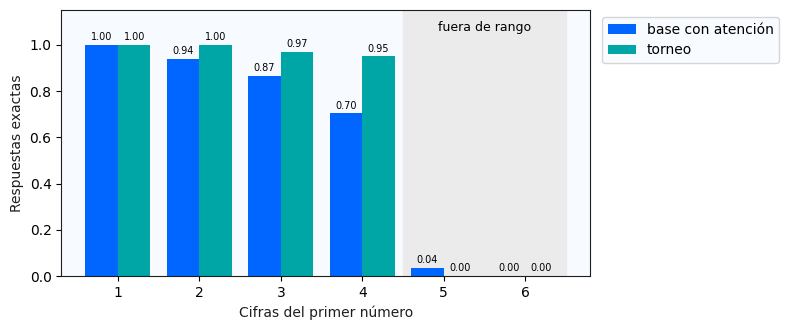
\includegraphics[width=.73\textwidth]{../artifacts/figuras/05_exactitud_base_vs_torneo.png}
\end{center}
\end{slide}

\begin{slide}{05 · ¿Dónde ayuda la atención?}
\begin{minipage}{.6\textwidth}
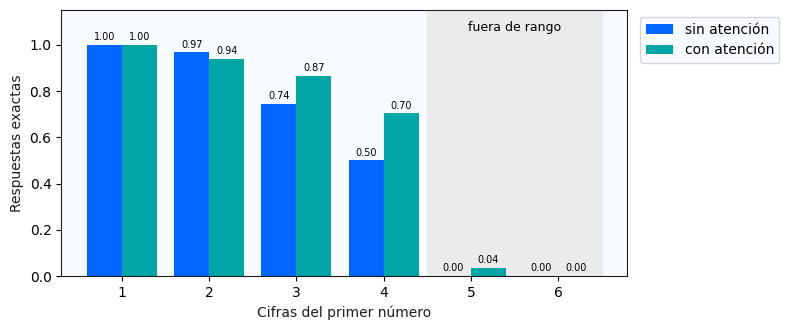
\includegraphics[width=\textwidth]{../artifacts/figuras/03_exactitud_por_cifras_baselines.png}
\end{minipage}\hfill
\begin{minipage}{.35\textwidth}
{\Large\color{ElectricBlue}\bfseries Cuatro cifras}\par
\vspace{.2cm}
Atención: \textbf{70.33\%}\par
Contexto fijo: \textbf{50.00\%}\par
Ventaja: \textbf{+20.33 pp}\par
\vspace{.35cm}
Con secuencias cortas, un resumen fijo todavía retiene información. Al crecer la entrada, la selección
dinámica reduce el cuello de botella.
\end{minipage}
\end{slide}

\begin{slide}{06 · Atención no significa algoritmo}
\begin{center}
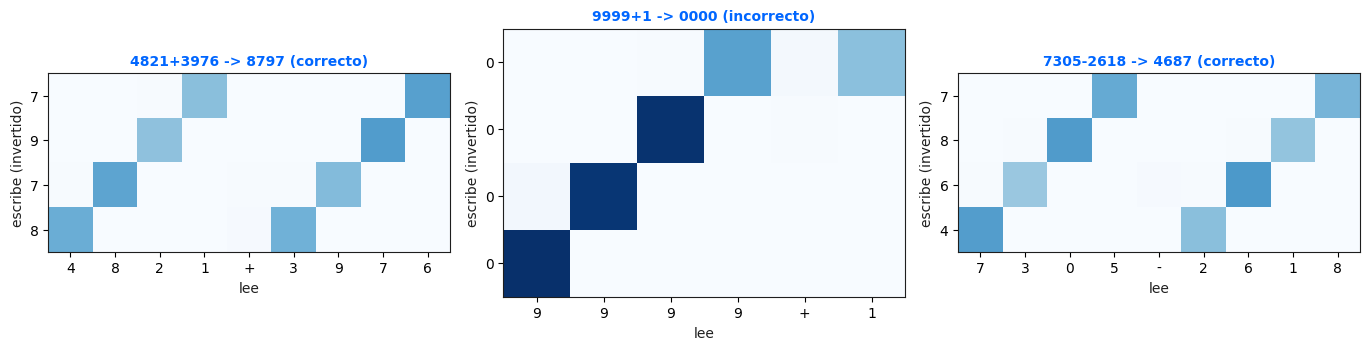
\includegraphics[width=.84\textwidth]{../artifacts/mapas_atencion/06_atencion_torneo.png}
\end{center}
\begin{itemize}
\item La alineación cambia con cada dígito generado.
\item La salida invertida sigue el sentido natural del acarreo.
\item El mapa aporta interpretación, pero no demuestra una regla simbólica causal.
\end{itemize}
\end{slide}

\begin{slide}{07 · Cinco formas de romperlo}
\begin{minipage}{.48\textwidth}
\begin{tabular}{lrr}
\toprule Problema & Predicción & Correcta \\
\midrule
\texttt{9999+1} & \texttt{0000} & \texttt{10000} \\
\texttt{9998+2} & \texttt{0000} & \texttt{10000} \\
\texttt{9999+9999} & \texttt{18998} & \texttt{19998} \\
\texttt{1000-999} & \texttt{11} & \texttt{1} \\
\texttt{4000-3999} & \texttt{001} & \texttt{1} \\
\bottomrule
\end{tabular}
\vspace{.4cm}
Fallan cambios de longitud, acarreos globales, préstamos por ceros y supresión de ceros iniciales.
\end{minipage}\hfill
\begin{minipage}{.48\textwidth}
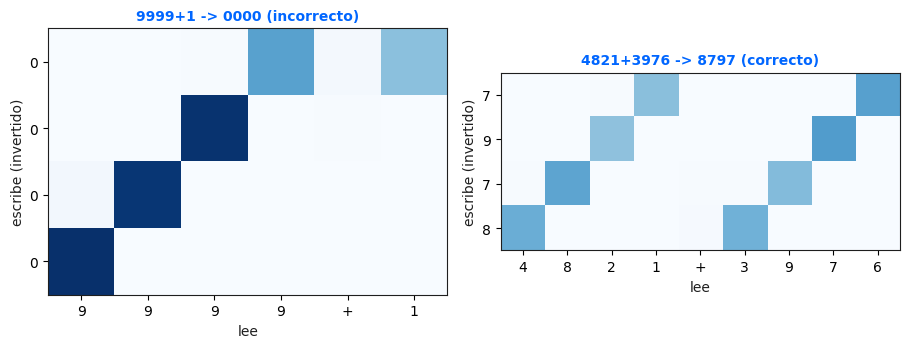
\includegraphics[width=\textwidth]{../artifacts/mapas_atencion/07_trampa_vs_control.png}
\end{minipage}
\end{slide}

\begin{slide}{08 · Repositorio reproducible}
\begin{minipage}{.48\textwidth}
\begin{verbatim}
notebooks/    original + final ejecutado
modelos_lab6/ tres checkpoints congelados
tareas/       documentación por bloque 0-7
artifacts/    métricas, figuras y validación
scripts/      construcción y controles
informe/      fuente TeX + PDF
presentacion_repositorio/ fuente TeX + PDF
\end{verbatim}
\end{minipage}\hfill
\begin{minipage}{.47\textwidth}
\begin{enumerate}
\item Construir desde el machote.
\item Ejecutar descubrimiento.
\item Integrar métricas y trampas.
\item Ejecutar versión final.
\item Exportar figuras.
\item Validar rúbrica y artefactos.
\end{enumerate}
\end{minipage}
\vspace{.4cm}
\fcolorbox{ElectricBlue}{SoftBlue}{\parbox{.93\textwidth}{
\textbf{Trazabilidad:} huella \texttt{94e198ec75ec}; 16 celdas ejecutadas y checkpoint sin reentrenar.}}
\end{slide}

\begin{slide}{09 · Resultado oficial del torneo}
\begin{center}
\card{80.5/100}{puntaje total}\hfill
\card{40/40}{acarreos en cadena}\hfill
\card{0/15}{jefe final · 5 cifras}
\end{center}
\vspace{.55cm}
\begin{itemize}
\item Clave oficial: \texttt{5978}; 53 respuestas exactas de 66.
\item Calentamiento: 20/20; cuatro cifras: 17/20; acarreos: 16/16; jefe final: 0/10.
\item El formulario confirmó el envío de las respuestas del torneo.
\item El checkpoint fue cargado directamente; no se ejecutó entrenamiento.
\item Huella antes y después: \texttt{94e198ec75ec}.
\item El resultado confirma fortaleza en acarreos y límite de extrapolación.
\end{itemize}
\vfill
\begin{center}\Large
\href{https://github.com/DanielBarillasM/Laboratorio-6_Daniel-Barillas_22193_DLYSI_Sec-30}{\textcolor{ElectricBlue}{Repositorio completo en GitHub}}
\end{center}
\end{slide}

\end{document}
